\chapter{車線変更時刻推定法}\chaplab{methods}
前章では,車線変更前の前方車両との距離,速度を用いて得られた成分が,二次元の正規分布に従っていると考えられることを示した.本章においては,この仮定を用いて,逐次的に車線変更を行う時刻を推定する手法について解説する.まず,逐次ベイズ推定による時系列データ%嘘
の一般的な扱いや,正規分布の定義から尤度関数を導出する方法について述べる.次に,事前分布の仮定や,尤度関数による事後分布の更新方法を述べる.最後に,実際に運転行動データに適用する際に設定したパラメータや諸手続きの詳細について述べる.
\section{逐次ベイズ推定}
車線変更開始時点を原点としたときの現在の時刻を$\tau$($T$以上の負の整数)と置く.はじめに,$\tau$に属する正規分布を$T\times N$次元のデータ行列$\mathbfcal{D}_\mathit{train}$から求める.$\mathbfcal{D}_\mathit{train}$の要素$\mathbf{x}_{\tau,n}$は,観測により得られた各特徴のベクトルとなっている.また,ある観測の系列を$\mathcal{D}_n$とおく.以下,$T=-20$, $N=2$と考え,$\mathbf{x}=\{\lambda_1, \lambda_2\}$とする.
\par
$\mathbfcal{D}_\mathit{train}$から,各時刻$\tau$に属する正規分布$\mathcal{N}_\tau$を求める.まず,二次元の正規分布は
\begin{align}
	\mathcal{N}(\xvec|\muvec,\Sigmavec)=\frac{1}{2\pi\detSigmavec^{1/2}}\exp\left\{-\frac{1}{2}(\xvec-\muvec)^\mathrm{T}\Sigmavec^{-1}(\xvec-\muvec)\right\}
\end{align}
と書ける.ただし,$\muvec$は2次元の平均ベクトル,$\Sigmavec$は$2\times2$の共分散行列,$\detSigmavec$は$\Sigmavec$の行列式である.$\mathcal{N}_\tau$の平均$\muvec_\tau$,共分散行列$\Sigmavec_\tau$を最尤推定で求めると,
\begin{align}
	\muvec_\tau&=\frac{1}{N}\sum_{n=1}^N \mathbf{x}_n\\
	\Sigmavec_\tau&=\frac{1}{N-1}\sum_{n=1}^N (\mathbf{x}_{\tau,n}-\muvec_{\tau})(\mathbf{x}_{\tau,n}-\muvec_\tau)^\mathrm{T}
\end{align}
となる.それぞれ,サンプルの平均,不偏分散に等しい.
訓練データから平均,分散を求める仮定を図示したものが,\figref{training_flow}である.
\begin{figure}[htbp]
  \centering
    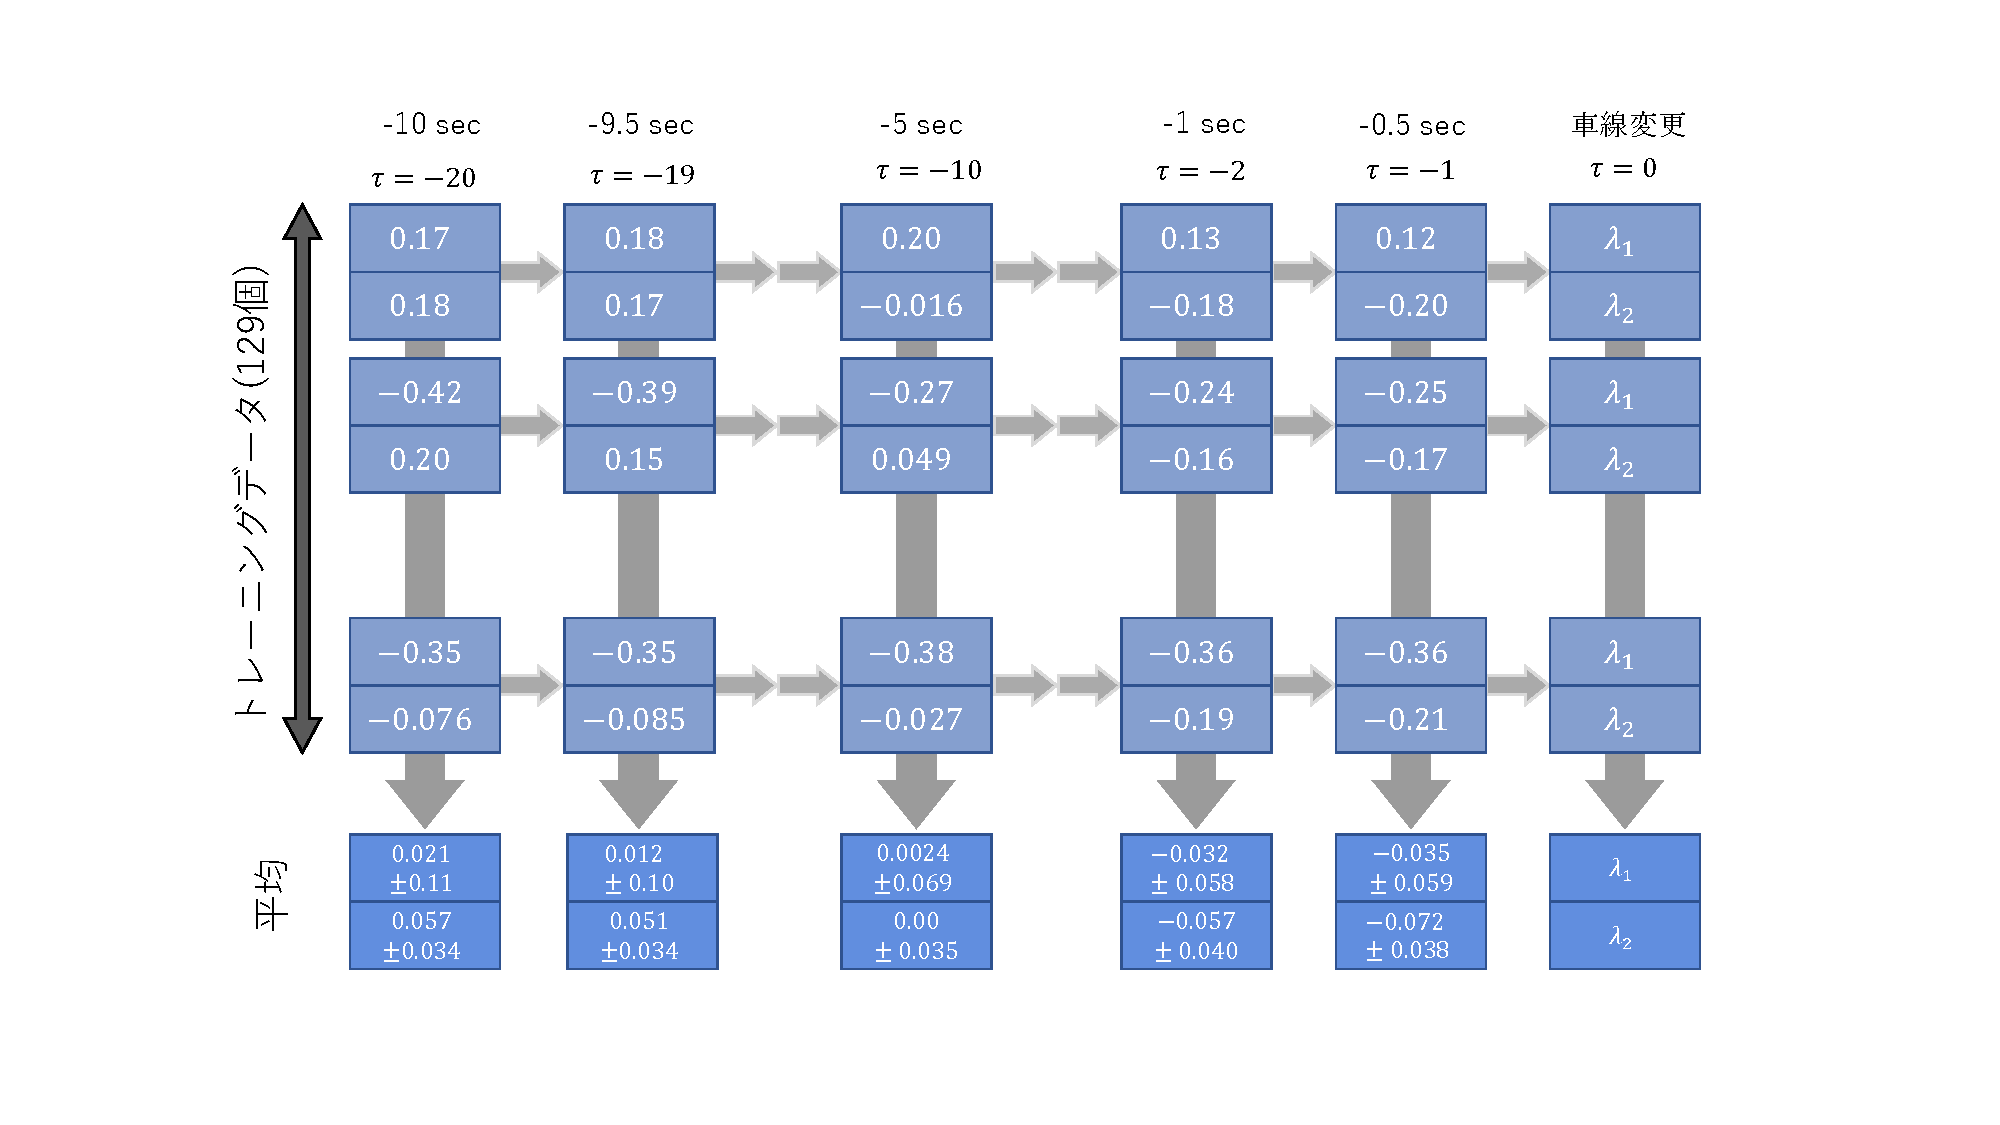
\includegraphics[width=11cm,keepaspectratio]{fig/training_flow.pdf}
  \caption{正規分布を訓練データからる流れを図示したもの.各セルの中の値は特徴量$\lambda_1$, $\lambda_2$の一例を示している.各行はある車線変更の1試行において得られた特徴の推移を並べており,これらの129回分について平均,分散を求めることで,各時刻の属する正規分布を求めている.}
  \label{fig:training_flow}
\end{figure}

トレーニングデータ129個を各時刻ごとにまとめ,平均,分散を出力することで,各時刻が属する正規分布を得ている.
\par
次に,$\tau$に対し事前分布をおき,正規分布から与えられる尤度によって車線変更開始までの時間を逐次的に更新することを考える.自車両と周辺車両の関係についての観測値が与えられていない時,$\tau$は一様分布であると仮定する.この時事前分布は
\begin{align}
p(\tau)=1/T
\end{align}
と表される.
\par
観測値が得られた時,時刻$\tau$に対する確率分布$p(\tau)$を更新する.観測値$\mathbf{x}_1$が得られたときの尤度は
\begin{align}
	p(\tau|\mathbf{x}_1)=\mathcal{N}(\xvec_1|\muvec_\tau,\Sigmavec_\tau)
\end{align}
となる.よって一度目の更新で得られる事後分布$p(\tau|\mathbf{x}_1)$は以下のように表される.
\begin{align}
	p(t|\xvec_1)\propto p(\xvec_1|\tau)p(\tau-1)=\frac{1}{N}\frac{1}{2\pi\detSigmavec_\tau^{1/2}}\exp\left\{-\frac{1}{2}(\xvec_1-\muvec_\tau)^\mathrm{T}\Sigmavec_\tau^{-1}(\xvec_1-\muvec_\tau)\right\}
\end{align}
ここで,時刻$\tau$となる確率が$p(\tau-1)$に依存している.これは,新しい観測値を得るまでに0.5秒の時間が経過しているため,0.5秒前における分布と現在の尤度を掛けあわせている.また,更新により得られる事後分布は$\int p(\tau)dt=1$を満たしていないため,$\sum_\tau p(\tau|\xvec_1)$ですべての値を割ることで正規化を施す必要がある.
この更新の過程を図示したものが,\figref{update_flow}である.
\begin{figure}[htbp]
  \centering
    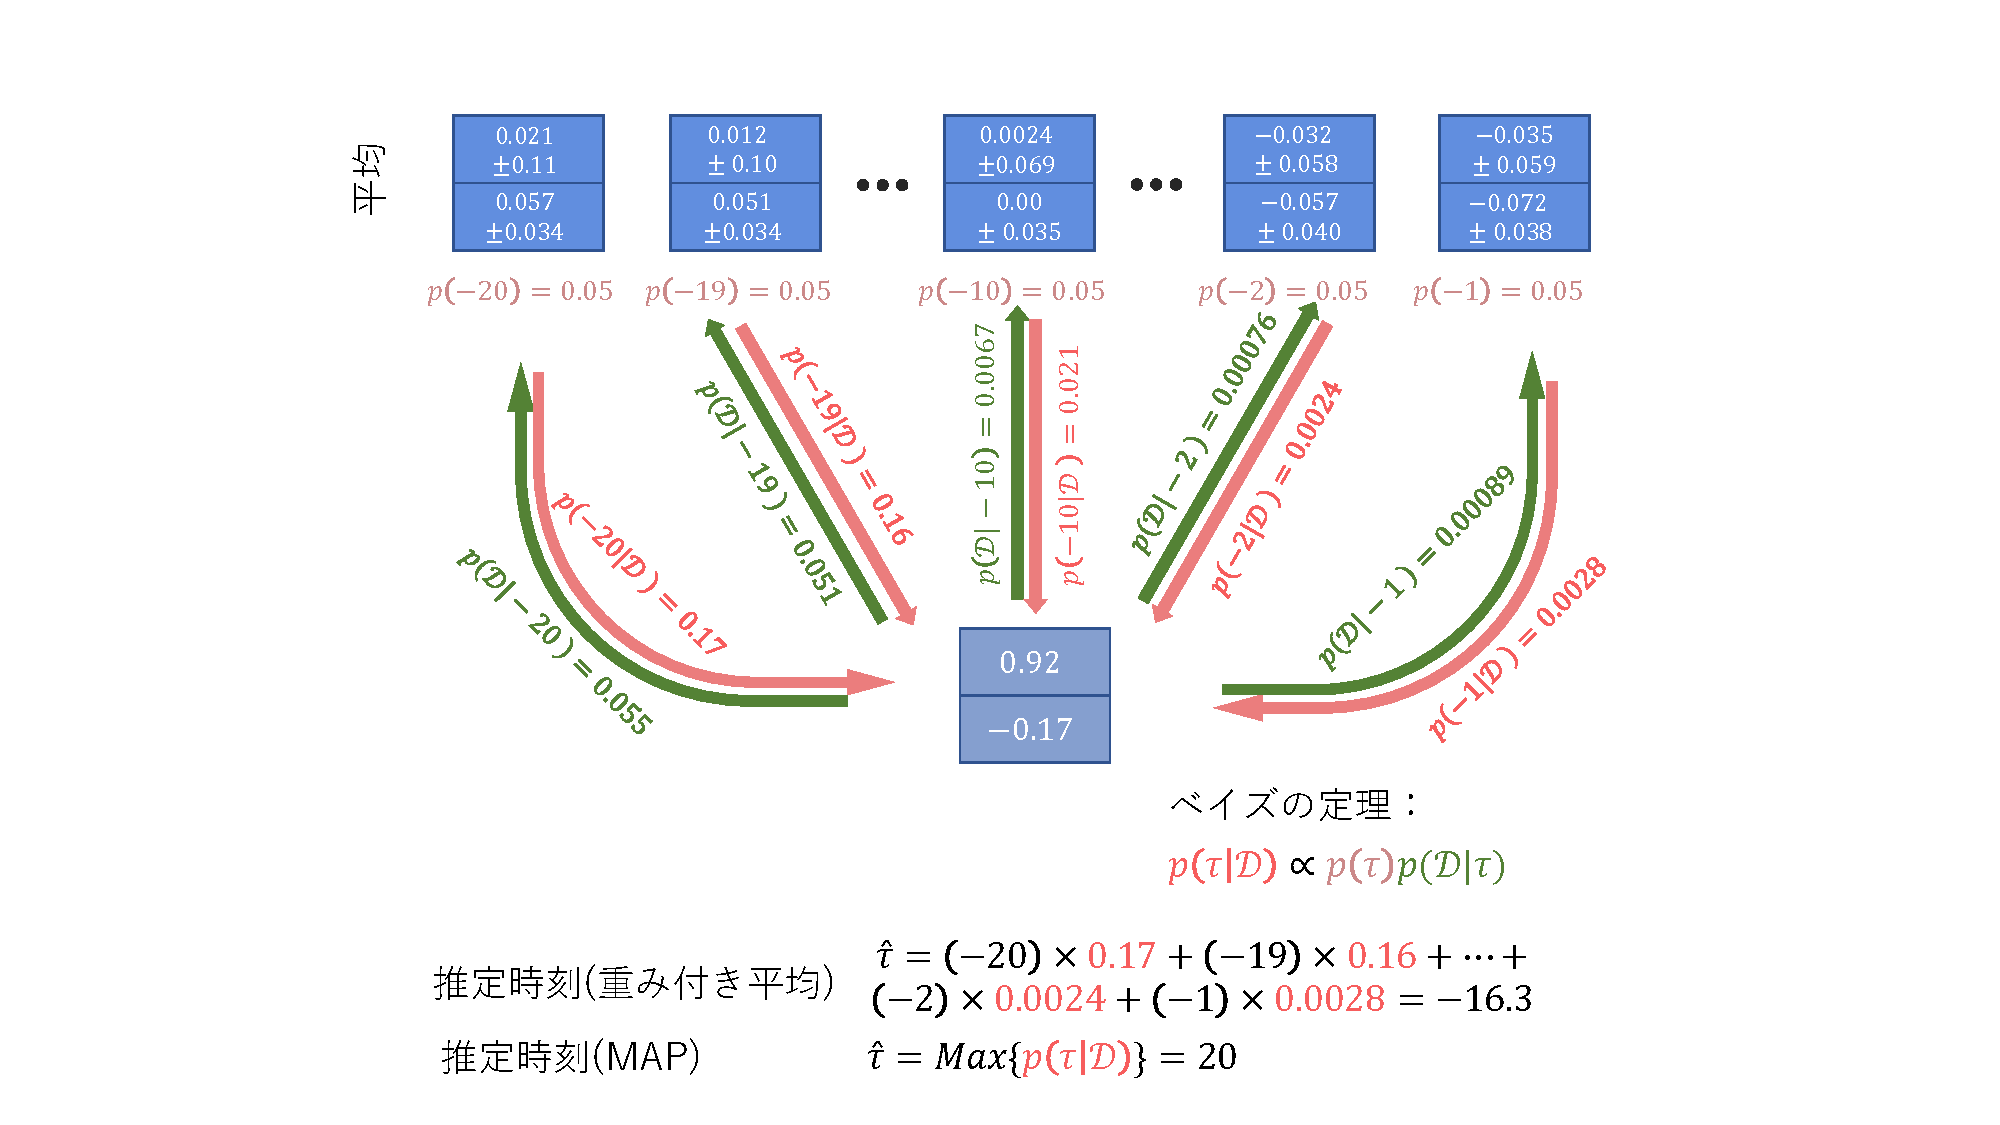
\includegraphics[width=11cm,keepaspectratio]{fig/update_flow.pdf}
  \caption{各時刻に属する正規分布から,現在の観測の尤度を求め,ベイズの定理により観測が得られたあとの分布を計算する様子を図示したもの.オレンジは事前分布,緑が尤度で,赤が事後分布を表している.また,図示した特徴量での例として,重み付き平均,MAPによる推定結果が幾つになるのかを示した.}
  \label{fig:update_flow}
  % figとfigure統一したかった
\end{figure}

ある観測点が得られたとき,その観測点が各時刻にどれだけ尤もらしいかを計算し,各時刻である確率分布を更新している.
\par
この更新の結果を一般化し,$k$回観測値を得られたときのデータ集合$\mathcal{D}_k=\{\xvec_1,\ldots,\xvec_k\}$から事後分布を求める.一度の観測で一単位時間が動くことを考えると,事後分布$p(\tau|\mathbf{x}_1)$は以下のように表される.
\begin{align}
	p(\tau|\mathcal{D}_k)\propto\frac{1}{N}\prod_{i=1}^k \mathcal{N}(\xvec_i|\muvec_{\tau-i+k}, \Sigmavec_{\tau-i+k})
\end{align}
例えば,3回分の観測データが与えられたとき,$\tau=-5$となる確率を求めるには,一つ目の観測が得られたときに$\tau=-7$となる尤度を,二つ目の観測が得られたときに$\tau=-6$となる尤度を,そして3回目のデータが得られたときに$\tau=-5$となる尤度を計算して掛け合わせればよい.
\par
以上が車線変更時刻の推定のために用いた逐次ベイズ推定の方法である.
\section{実計算での手続きやパラメータ設定}
計算上では,尤度を掛け合わせていくと非常に小さな値となってしまい誤差が発生してしまうため,実際は対数尤度の和を用いて計算を行った.%ここ詳しく書く?
$\xvec_\tau$については,時刻$\tau$のときの周辺車両との相対位置,相対速度と,$\tau-1$のときの周辺車両との相対位置,相対速度の4次元ベクトルに対し.主成分分析によって2次元に落とし込んだものを観測値としている.
\par
また,すべての右車線変更161回のうち,$4/5$にあたる129回を訓練データに,$1/5$に当たる32回をテストデータとした.訓練データを主成分分析にかけ,各$\tau$の属する正規分布を導出した後,テストデータにも訓練データにより得られた変換を施し,変換を施したテストデータを用いて上述のベイス推定を行い,各時刻の推定結果を重み付き平均,MAP推定の2つの方法で導出した.
